\documentclass[12pt,letterpaper]{report}

% Required packages
\usepackage{geometry}
\usepackage{titlesec}
\usepackage{titling}
\usepackage{hyperref}
\usepackage{pdfpages}
\usepackage{fancyhdr}
\usepackage{lastpage}
\usepackage{graphicx}
\usepackage{enumitem}
\usepackage{xcolor}

% Page formatting
\geometry{margin=1in}
\pagestyle{fancy}
\fancyhf{}
\renewcommand{\headrulewidth}{0pt}
\fancyfoot[C]{\thepage}
\setcounter{secnumdepth}{0}

% Custom section formatting
\titleformat{\chapter}[display]
{\normalfont\Huge\bfseries\centering}{\chaptertitlename\ \thechapter}{20pt}{\Huge}
\titlespacing*{\chapter}{0pt}{50pt}{40pt}

% Define colors
\definecolor{vanderbiltgold}{RGB}{216,171,76}
\definecolor{vanderbiltblack}{RGB}{0,0,0}

% Custom commands for section dividers
\newcommand{\sectiondivider}[1]{%
    \clearpage
    \thispagestyle{empty}
    \begin{center}
        \vspace*{\fill}
        {\Huge\bfseries\textcolor{vanderbiltblack}{#1}}
        \vspace*{\fill}
    \end{center}
    \clearpage
}

% Document metadata
\title{Master of Science in Computer Science\\Non-Thesis Portfolio}
\author{Haoli Yin}
\date{\today}

\begin{document}

% Cover page
\begin{titlepage}
    \centering
    \vspace*{0.5cm}
    {
\includegraphics[width=0.3\textwidth]{vanderbilt_logo.pdf}\par}
    \vspace{0.7cm}
    {\LARGE\bfseries Master of Science in Computer Science\par}
    \vspace{0.5cm}
    {\LARGE\bfseries Non-Thesis Portfolio\par}
    \vspace{0.7cm}
    {\Large\textbf{Haoli Yin}\par}
    \vspace{0.2cm}
    {\normalsize\textbf{Commodore ID: }000768997\par}
    \vspace{0.2cm}
    {\normalsize\textbf{VUNetID: }yinh4\par}
    \vspace{0.2cm}
    {\normalsize\textbf{Masters Start:} Fall 2023\par}
    \vspace{0.2cm}
    {\normalsize\textbf{Expected Graduation:} Spring 2025\par}
    \vspace{0.7cm}
    {\normalsize\textbf{Academic Advisor}\par}
    \vspace{0.2cm}
    {\normalsize Dr. Tyler Derr\par}
    \vspace{0.7cm}
    {\normalsize\textbf{Advisor Signature}\par}
    \vspace{0.2cm}
    \begin{center}
        \rule{7cm}{0.4pt}
    \end{center}
    \vspace{0.4cm}
    {\normalsize\textbf{Date}\par}
    \vspace{0.2cm}
    \begin{center}
        \rule{7cm}{0.4pt}
    \end{center}
    \vspace{0.7cm}
    {\normalsize\textbf{Department of Computer Science}\\
    \textbf{School of Engineering}\\
    \textbf{Vanderbilt University}\par}
    \vspace{0.5cm}
    {\normalsize\today\par}
\end{titlepage}

% Table of Contents
\tableofcontents
\clearpage

% Section 1: Summary Data
\sectiondivider{Summary Data}
\chapter{Summary Data}

\section{Personal Information}
\begin{itemize}
    \item \textbf{Name:} Haoli Yin
    \item \textbf{Date Entered Program:} Fall 2023
    \item \textbf{Status:} Full Time
    \item \textbf{Principal Source of Support:} Cornelius Vanderbilt Scholarship
\end{itemize}

\section{Academic Advisor}
\begin{itemize}
    \item \textbf{Name:} Dr. Tyler Derr
\end{itemize}

\section{Courses and Grades}

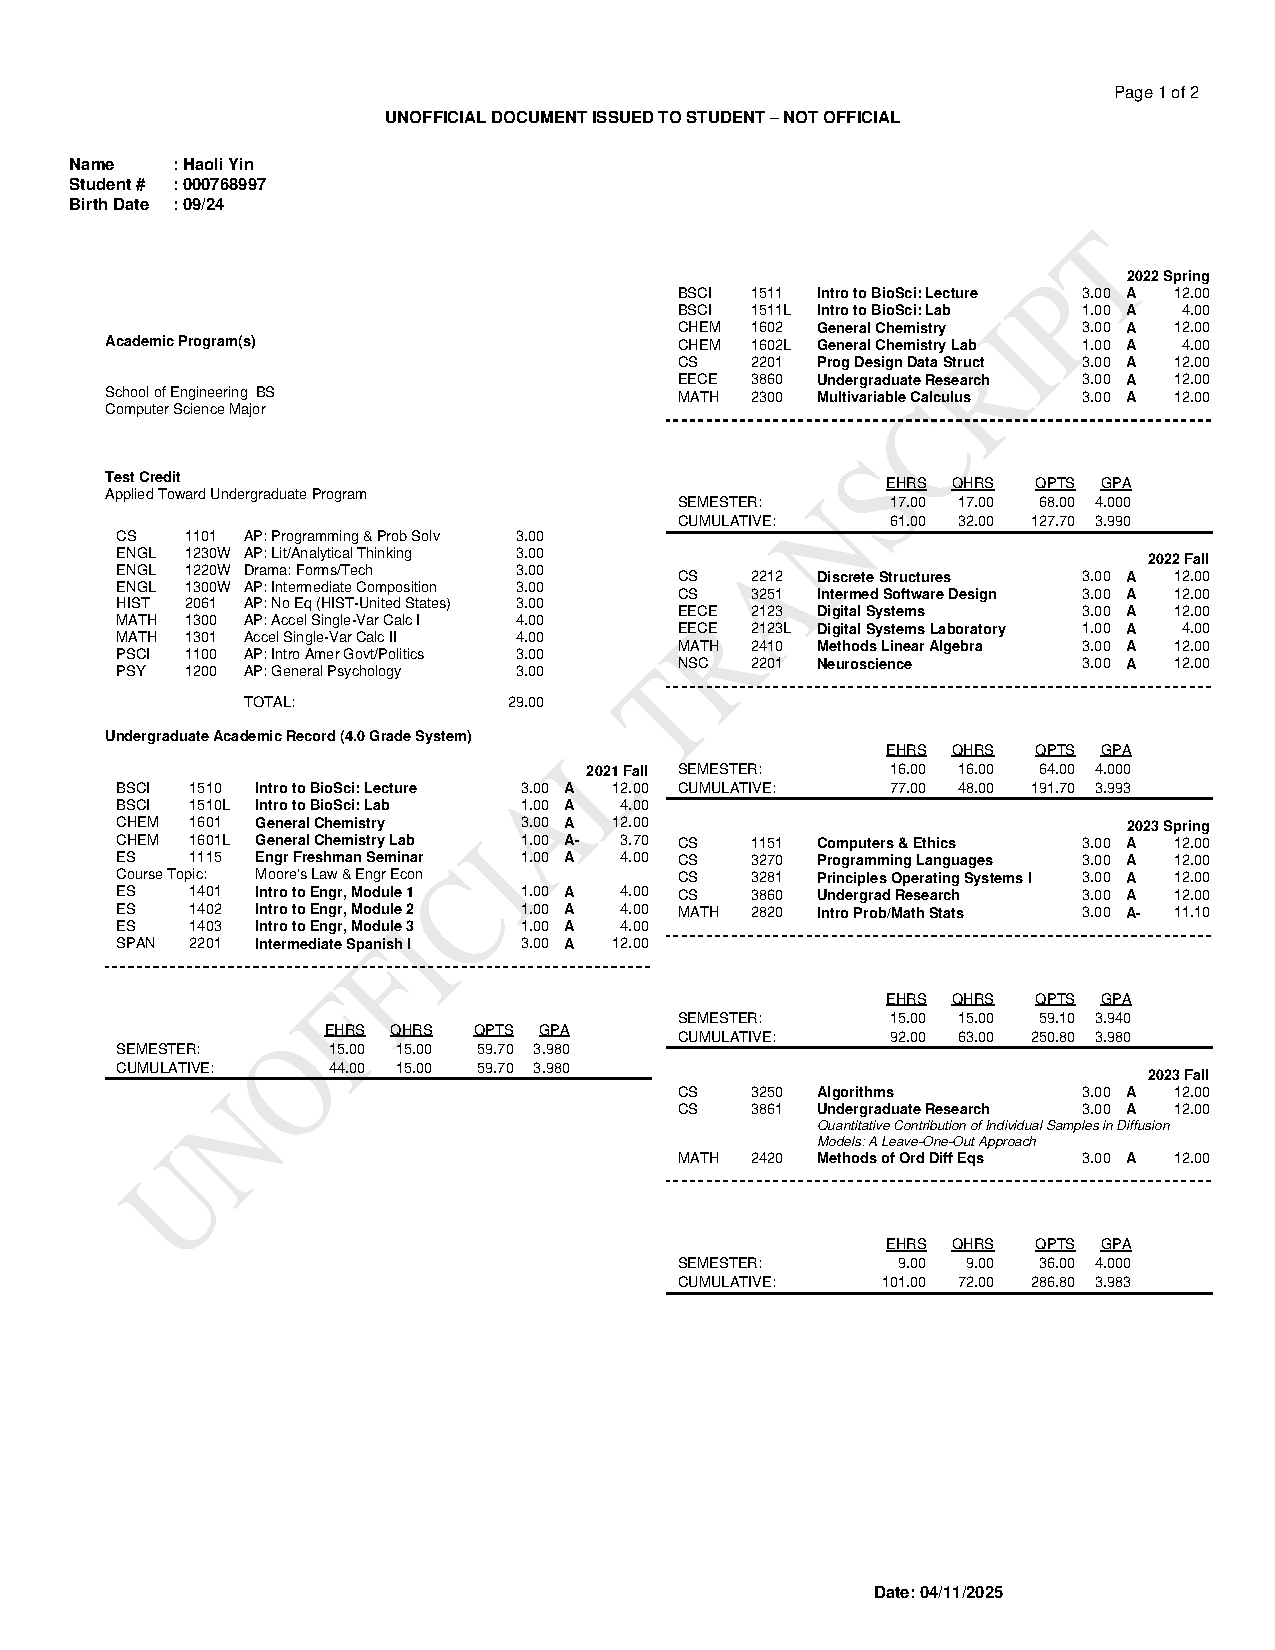
\includepdf[pages=-, scale=1.0, pagecommand={\thispagestyle{fancy}}]{spring2025transcript.pdf}

% Section 2: Statement of Professional Goals and Achievements
\sectiondivider{Statement of Professional Goals and Achievements}
\chapter{Statement of Professional Goals and Achievements}

\section{Professional Goals}
My journey in computer science has shaped ambitious yet focused professional aspirations that blend technical innovation with real-world impact. I aim to advance large-scale machine learning infrastructure, with particular emphasis on vision-language systems that can transform how humans interact with technology. Specializing in distributed computing solutions for extremely large-scale deployments (100TB+), I seek to address fundamental challenges in data processing that arise at the intersection of different modalities.

At the heart of my professional goals is a commitment to making multimodal systems more efficient and accessible. My master's degree has equipped me with both the theoretical foundation and practical experience to tackle complex problems in this domain, preparing me to contribute meaningfully to research teams and industry projects that push the boundaries of what's possible in machine learning and distributed systems.

\section{Achievements During Graduate Studies}
During my graduate studies, I've been fortunate to engage in research and professional experiences that have significantly shaped my development as a computer scientist. I've authored several impactful publications, including ``UniCat: Crafting a Stronger Fusion Baseline for Multimodal Re-Identification,'' which was accepted at the NeurIPS 2023 UniReps Workshop and achieved state-of-the-art performance on several benchmark datasets. Additionally, my work on ``GraFT: Gradual Fusion Transformer for Multimodal Re-Identification'' received borderline acceptance at WACV 2024, representing the culmination of my research internship at Modern Intelligence.

My research in biomedical applications has been particularly rewarding, with projects like ``Digital Staining of Unpaired White and Blue Light Cystoscopy Videos for Bladder Cancer Detection'' and ``SpecReFlow: A Specular Reflection Restoration Framework.'' The latter allowed me to deliver an oral presentation at the SPIE Photonics West 2023 Conference.

Professionally, I've made significant contributions at organizations like DatologyAI, where I orchestrated data pipelines at multi-billion sample scale and improved CLIP pretraining efficiency by over 10x. At Modern Intelligence, I led the development of novel multimodal fusion techniques while enhancing the team's infrastructure for model training, achieving a 400\% improvement in training speed.

My academic achievements have been recognized through prestigious honors, including being named a Neo Scholar Finalist (2024), receiving the Goldwater Scholarship (2023), participating in the Google CS Research Mentorship Program, and maintaining my Cornelius Vanderbilt Scholarship throughout my studies.

\section{Interests in Computer Science}
I'm drawn to the fascinating intersection of systems engineering and machine learning, where theoretical advancements meet practical implementation challenges. This space offers abundant opportunities to solve meaningful problems that impact how we process, understand, and derive value from data at scale.

My passion centers on addressing scale challenges in multimodal processing—finding elegant solutions to the computational and architectural problems that arise when working with diverse data types simultaneously. The complexity of these systems, with their intricate performance trade-offs and optimization requirements, presents intellectually stimulating puzzles that I find deeply engaging.

My academic journey has followed a deliberate path from cloud computing foundations to advanced machine learning techniques. This progression has allowed me to build a comprehensive understanding of both the infrastructure that supports AI systems and the algorithms that drive them forward. Through coursework, research projects, and industry experience, I've cultivated expertise in distributed systems, optimization techniques, and multimodal fusion approaches that form the foundation of next-generation AI applications.

% Section 3: Curriculum Vitae
\sectiondivider{Curriculum Vitae}
\chapter{Curriculum Vitae}

% Placeholder for CV - will be included from external PDF
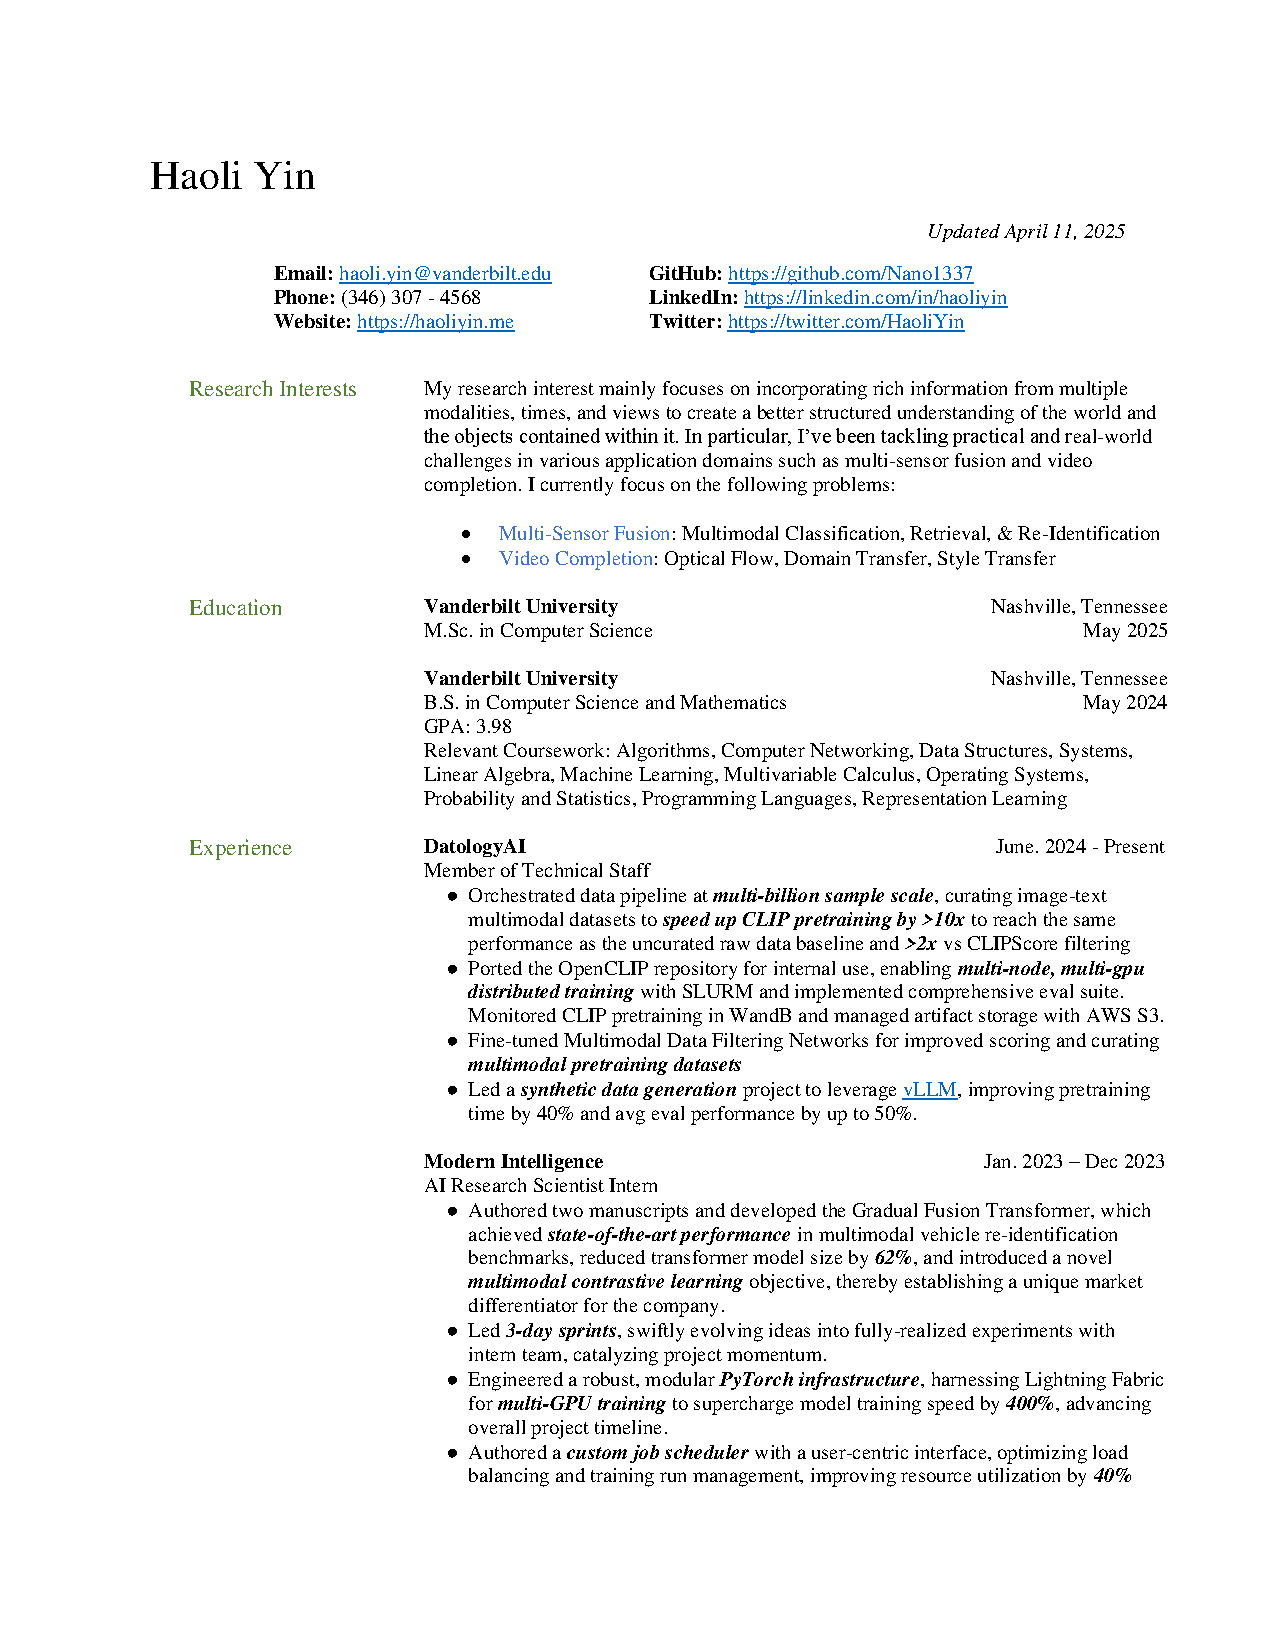
\includepdf[pages=-, scale=1.0, pagecommand={\thispagestyle{fancy}}]{Haoli_Yin_CV_2025.pdf}

% Uncomment the following line and provide the path to your CV when ready
% \includepdf[pages=-]{path/to/your/cv.pdf}

% Section 4: Knowledge and Mastery of Computer Science Concepts
\sectiondivider{Knowledge and Mastery of Computer Science Concepts}
\chapter{Knowledge and Mastery of Computer Science Concepts}

\section{Application of Computer Science Concepts}
Paper: "Unimodal Ensemble: Addressing Modality Laziness in Multimodal Fake News Detection" from the class AI for Cyberphysical Systems with Dr. Meiyi Ma. 

\subsection{Problem Statement}
% Replace with your problem statement
The paper addresses the challenge of "modality laziness" in multimodal fake news detection systems. This phenomenon occurs when multimodal models primarily learn from a dominant modality while underutilizing other modalities, leading to suboptimal performance. In multimodal fake news detection, where both textual and visual information are important for accurate classification, this bias significantly limits effectiveness, sometimes causing multimodal models to perform worse than unimodal alternatives.

\subsection{Methodology}
% Replace with your methodology
The authors propose a novel Unimodal Ensemble (UME) architecture that independently trains unimodal image and text models in parallel. Key aspects of the methodology include:

\begin{enumerate}
    \item Separate backbones for text and image processing, using transfer learning with pre-trained CLIP variants (SigLIP for Fakeddit dataset and Chinese CLIP for Weibo dataset)
    \item Independent training with modality-specific loss functions to ensure each modality learns its task-relevant features without cross-modal influence
    \item Simple averaging of unimodal logits during inference to create joint predictions
    \item Evaluation on two datasets: Fakeddit (English) and Weibo (Chinese)
\end{enumerate}

This approach intentionally avoids complex fusion mechanisms, focusing instead on maximizing the potential of each unimodal model before combination.


\subsection{Results and Discussion}
The UME architecture outperformed state-of-the-art multimodal fake news detection models (EANN, SpotFake, HMCAN, and CAFE) on both datasets:

\begin{itemize}
    \item Achieved highest accuracy on both Fakeddit (91.9%) and Weibo (92.7%) datasets
    \item Demonstrated superior performance for fake news detection metrics, with significant improvements in precision and recall
    \item Ablation studies confirmed UME's effectiveness compared to other approaches addressing modality laziness (late fusion, OGM-GE, and QMF)
\end{itemize}

The results suggest that allowing each modality to independently learn its optimal features before combination is more effective than traditional fusion-based approaches for multimodal fake news detection. The authors note this finding implies strong intra-modal signals for fake news detection exist within each modality separately, and that combining these signals through simple ensembling creates a more robust multimodal system.

\subsection{Personal Contribution}
As the primary technical contributor to this project, I led the implementation efforts across multiple phases. I developed the data pipeline for both the Fakeddit and Weibo datasets, including automated download scripts and preprocessing modules that standardized the multimodal inputs. For the model architecture, I implemented the parallel unimodal training approach with separate backbones for text and image processing, adapting pre-trained CLIP variants (SigLIP and Chinese CLIP) for our specific task. I also designed and executed the training framework with modality-specific loss functions, implemented the ensemble prediction mechanism, and created comprehensive evaluation protocols that measured performance across multiple metrics. Throughout the project, I maintained the codebase, ensuring reproducibility and documentation quality while collaborating with team members on experiment design and results analysis.

\section{Software Artifact}
\subsection{Project Overview}
% Replace with your project overview
The code linked below contains the full reproducible study for the paper. 

\subsection{Design}
The repository follows a modular architecture centered around reproducible machine learning workflows. The codebase is organized into distinct components for data processing, model training, and evaluation, with configuration files enabling experiment customization. This design facilitates independent training of unimodal models while maintaining a clean separation between preprocessing, feature extraction, and ensemble prediction mechanisms.
\textbf{GitHub Repository:} \url{https://github.com/Nano1337/ume-fakenews}

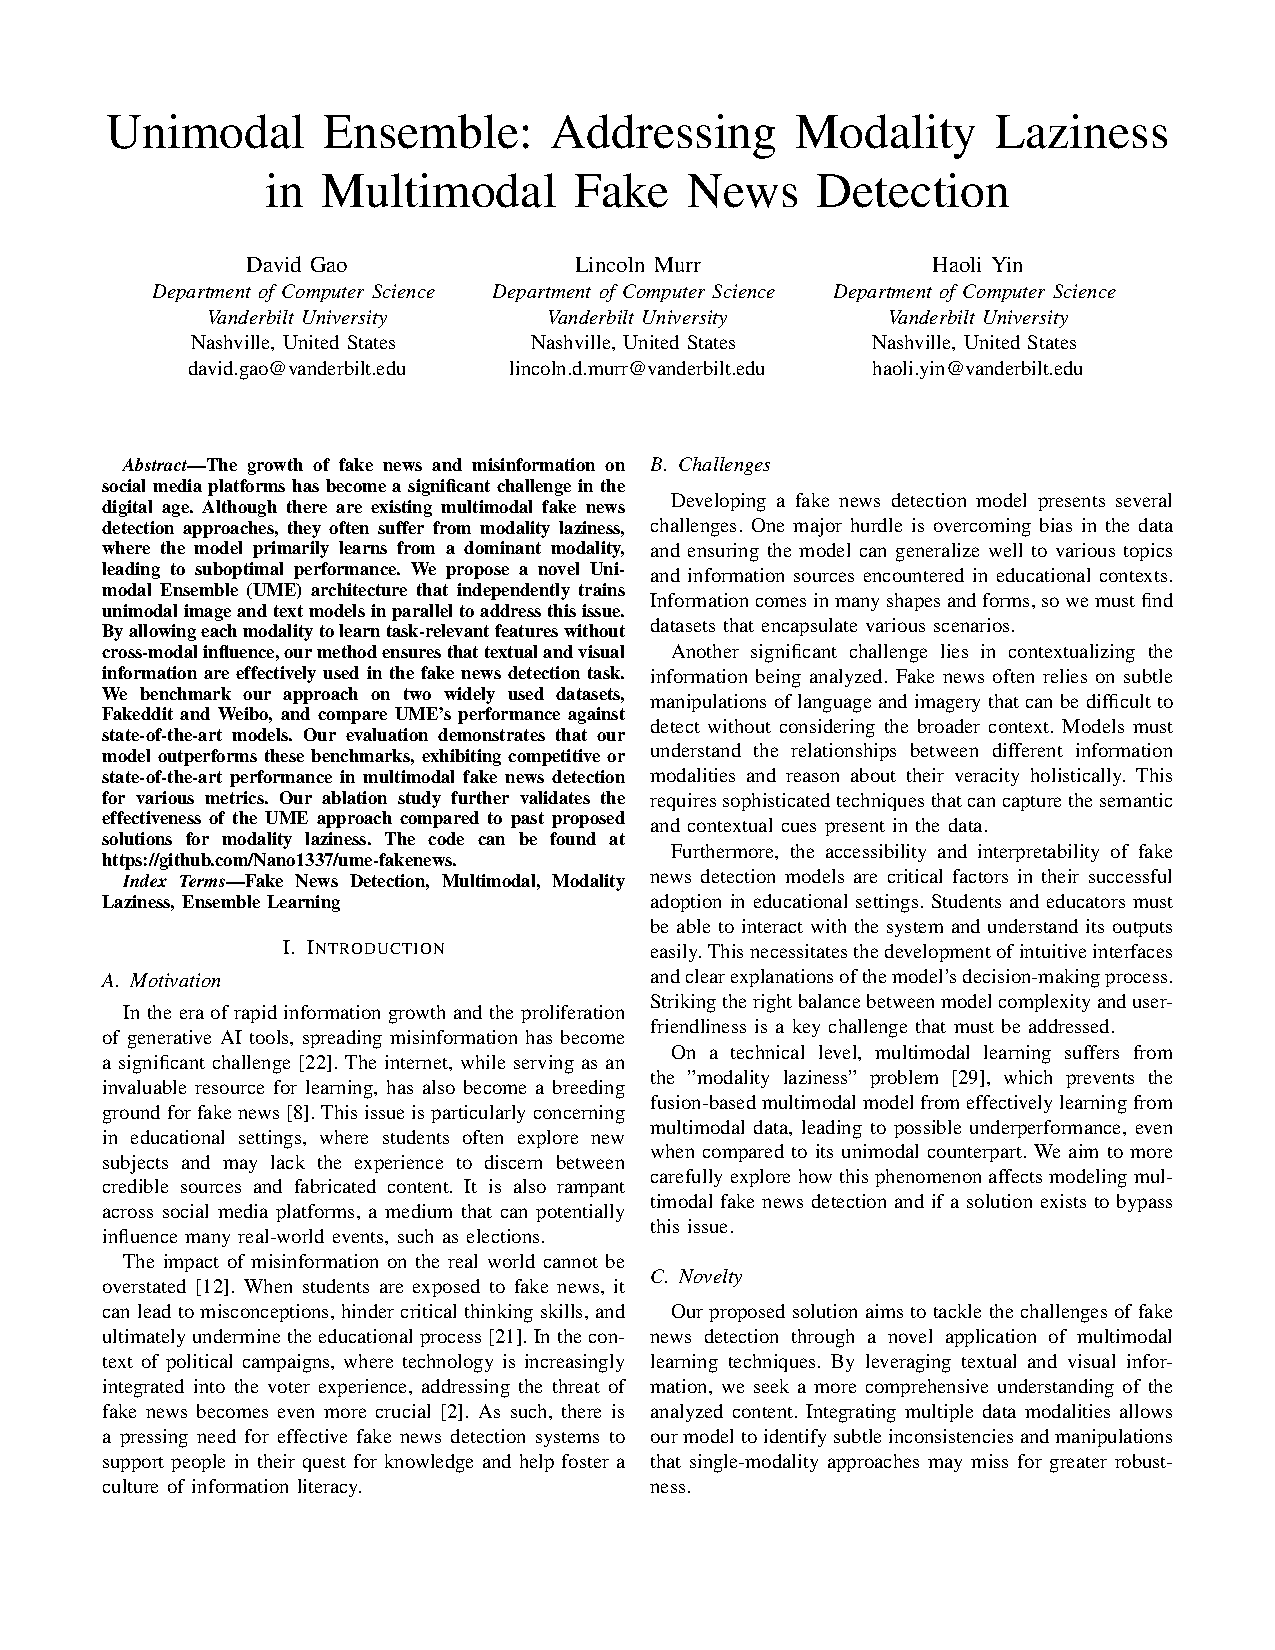
\includepdf[pages=-, scale=1.0, pagecommand={\thispagestyle{fancy}}]{ume-fakenews.pdf}

% Section 5: Communication Skills in Computer Science
\sectiondivider{Communication Skills in Computer Science}
\chapter{Communication Skills in Computer Science}

\section{Artifact Demonstrating Communication Skills}

\subsection{Context}
% Replace with context
This paper presentation was prepared for the graduate special topics class called "Security and Privacy in Pervasive Environments". 
The paper itself is called "Privacy Leakage via Unrestricted Motion-Position Sensors in VR: Snooping Typed Input on Virtual Keyboards" and was a study on privacy leakage in virtual reality environments.

\subsection{Slides Presentation}
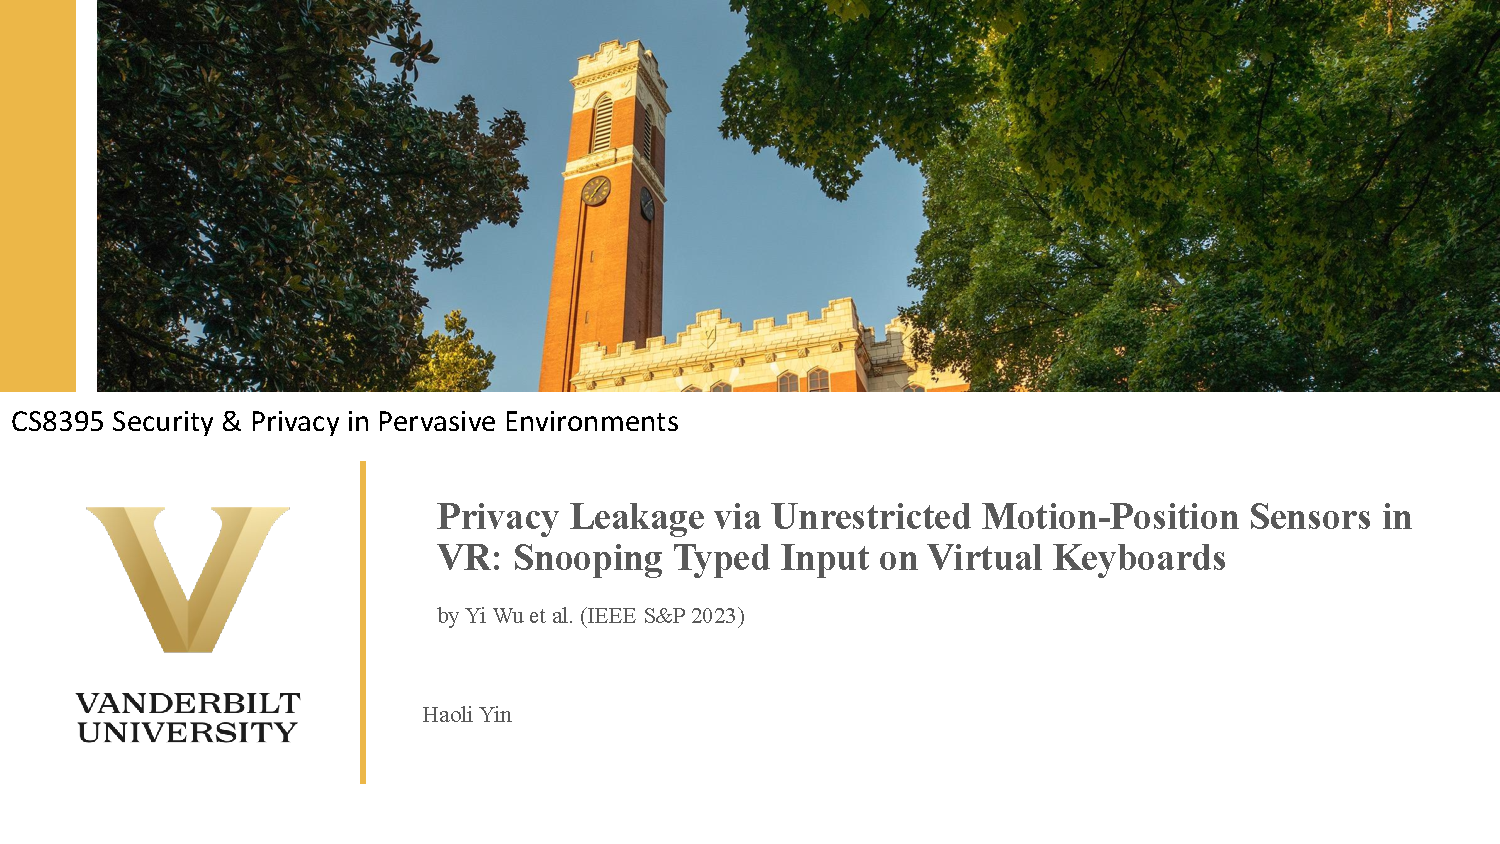
\includepdf[pages=-, scale=1.0, pagecommand={\thispagestyle{fancy}}]{privml.pdf}

% Section 6: Conduct Independent Inquiry in Computer Science
\sectiondivider{Conduct Independent Inquiry in Computer Science}
\chapter{Conduct Independent Inquiry in Computer Science}

\textbf{Paper Title:} SpecReFlow: An Algorithm for Specular Reflection Restoration Using Flow-Guided Video Completion

\textbf{Publication Details:} Journal of Medical Imaging, Volume 11, Issue 2, Pages 024012-024012, Society of Photo-Optical Instrumentation Engineers (SPIE), March 1, 2024.

\subsection{Problem Statement}
Specular reflections (SRs) are highlight artifacts commonly found in endoscopy videos that can severely disrupt a surgeon's observation and judgment. Despite numerous attempts to restore SR, existing methods are inefficient and time consuming and can lead to false clinical interpretations. Therefore, we propose the first complete deep-learning solution, SpecReFlow, to detect and restore SR regions from endoscopy video with spatial and temporal coherence.

\subsection{Research Methodology}
SpecReFlow consists of three stages: (1) an image preprocessing stage to enhance contrast, (2) a detection stage to indicate where the SR region is present, and (3) a restoration stage in which we replace SR pixels with an accurate underlying tissue structure. Our restoration approach uses optical flow to seamlessly propagate color and structure from other frames of the endoscopy video.

\subsection{Results and Findings}
Comprehensive quantitative and qualitative tests for each stage reveal that our SpecReFlow solution performs better than previous detection and restoration methods. Our detection stage achieves a Dice score of 82.8\% and a sensitivity of 94.6\%, and our restoration stage successfully incorporates temporal information with spatial information for more accurate restorations than existing techniques.

\subsection{Conclusions}
SpecReFlow is a first-of-its-kind solution that combines temporal and spatial information for effective detection and restoration of SR regions, surpassing previous methods relying on single-frame spatial information. Future work will look to optimizing SpecReFlow for real-time applications. SpecReFlow is a software-only solution for restoring image content lost due to SR, making it readily deployable in existing clinical settings to improve endoscopy video quality for accurate diagnosis and treatment.

\subsection{GitHub Repository}
\textbf{GitHub Repository:} \url{https://github.com/Nano1337/SpecReFlow}

\includepdf[pages=-, scale=1.0, pagecommand={\thispagestyle{fancy}}]{specreflow.pdf}

\end{document}
